位置情報を活用したルーティングプロトコルであるGPSRが正しく
機能するためには, 同一アドホックネットワーク内の
参加者が相互に正しい位置情報を送信する必要がある. 
しかし, ネットワーク内に不正なノードが存在する場合, 
ルーティングが妨害されかねない. この章では, 想定される 
不正ノードを示した後, その対策について述べる. \\

\noindent {\large\textbf{不正ノード}}\\[0.5em]
\noindent \textbf{1. 位置情報詐称ノード}\\
\indent 位置情報詐称ノードとは, 通信データの窃取を目的に, 
自身の位置情報を偽装してルーティングを妨害する内部不正ノードである. 
内部不正ノードとは, ネットワーク内において意図的に不正行為を行う
ノードのことで, 外部から侵入した攻撃者や, 内部の
信頼されたノードが乗っ取られることで発生することが一般的である. 
図\ref{fig:position-liar}のように, 送信ノード$S$が宛先ノード$D$に送信するとする. 
このとき, 本来$S$は電波伝搬範囲内で$D$に最も近い$A$を中継ノードとして
選択するべきであるが, ノード$B$が位置情報を詐称して$B'$の位置にいると
偽装することで, $B$を選択し, 誤ったルーティングをしてしまう. 
このようにして, $B$は本来$D$が受けるべきデータを窃取し, 
情報伝達を妨害できる.

\begin{figure}
  \centering
  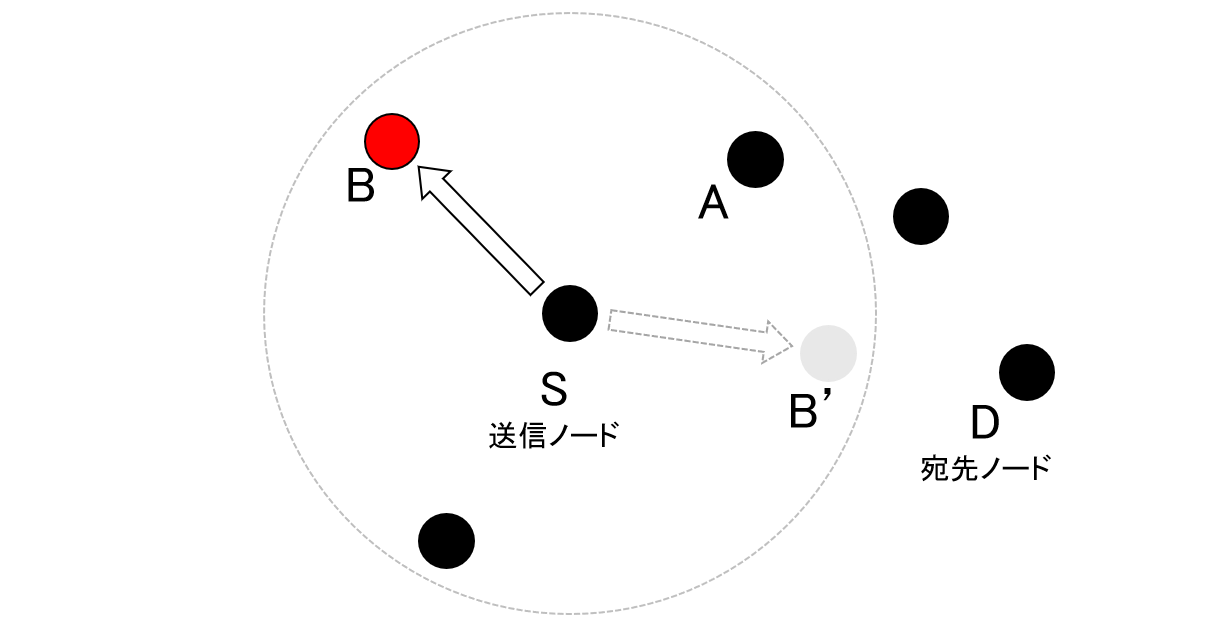
\includegraphics[scale=0.7]{figures/position-liar.png}
  \caption{位置情報詐称ノード}
  \label{fig:position-liar}
\end{figure}

\noindent \textbf{2. IPアドレス詐称ノード}\\
\indent IPアドレス詐称ノードとは, ネットワークへの不正アクセスを
目的とした外部不正ノードである. 外部不正ノードとは, ネットワークの
外部から侵入し, 不正な目的でネットワーク内のデータやリソースを
攻撃または利用しようとするノードのことである. 図\ref{fig:ip-liar}は,  
当該ネットワークの構成ノードを黒丸, 非構成ノードを赤丸で示している. 
赤丸で示した外部ノードがネットワーク内のIPアドレスを詐称して
ネットワーク参加者に送信した場合, その情報を受け取ったノードは
外部ノードを信頼し, 通信を行ってしまう. このように, 
IPアドレスを詐称することで外部ノードがネットワークに不正に
参加できてしまう. 

\begin{figure}
  \centering
  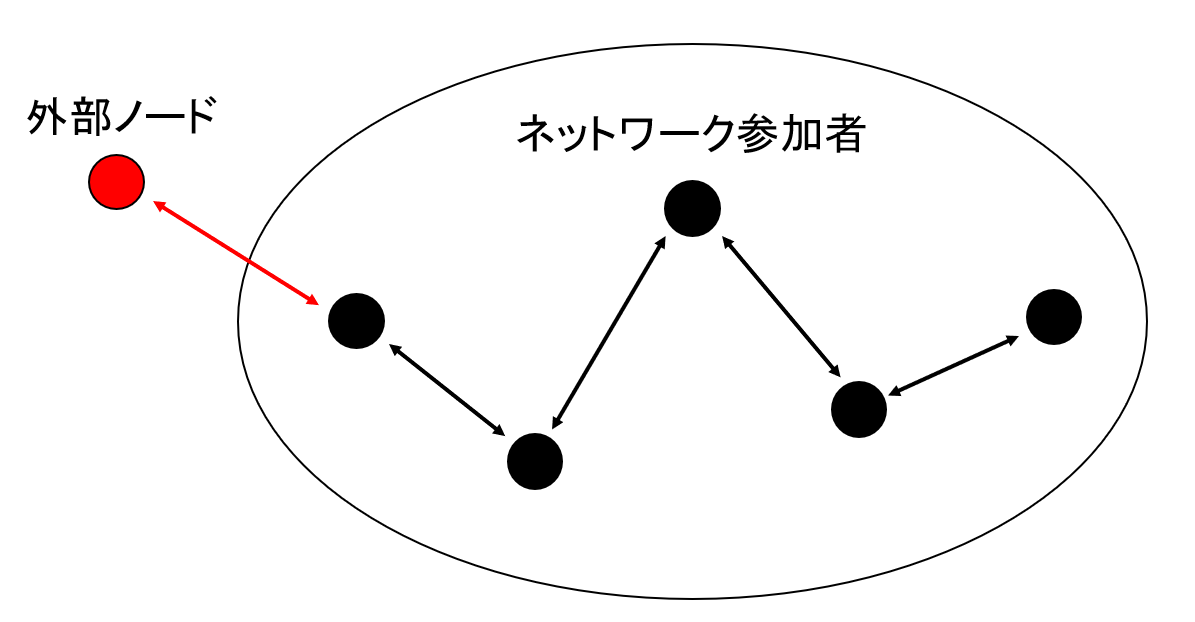
\includegraphics[scale=0.7]{figures/ip-liar.png}
  \caption{IPアドレス詐称ノード}
  \label{fig:ip-liar}
\end{figure}

\indent このような2種類の不正ノードが存在する場合, 正しいルーティングが
行われない. そこで, 本研究では, デジタル署名を用いてノードの情報が
正しいものであるかを検証し, なりすましや改ざんを排除するようにした. \\
\indent では, その仕組みを説明する. 図\ref{fig:signature-method}に示すように, 
ノード$A$からノード$B$にデータを送信する場合, $A$は認証局による
署名をデータに付与して$B$に送信する. 
$B$は受信したデータに対して署名の検証を行い, ネットワーク内の
正当なノードから正しいデータが送信されたかを確認する.
\newpage

\begin{figure}
  \centering
  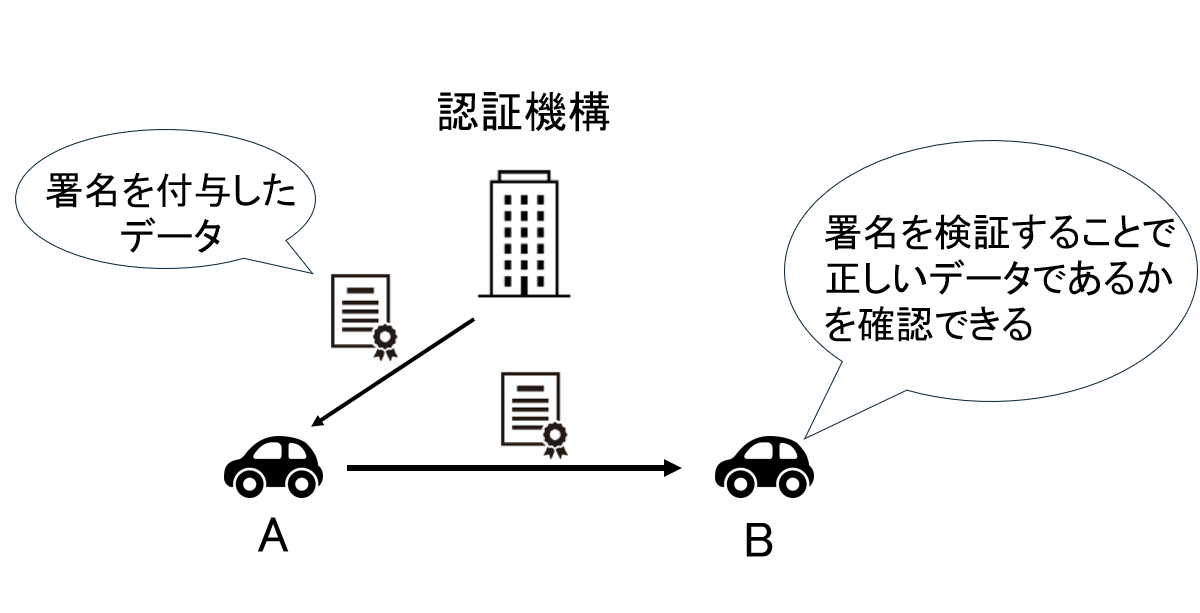
\includegraphics[scale=0.7]{figures/signature-method.png}
  \caption{本研究におけるデジタル署名の使用方法}
  \label{fig:signature-method}
\end{figure}

\indent 本研究で導入される認証機構は以下の通りである.
\setlength{\tabcolsep}{30pt}
\begin{longtable}{cc}
  \caption{認証機構(署名者)と被署名データの対応}
  \endfirsthead
  \hline
  \multicolumn{1}{c}{認証機構(署名者)} & \multicolumn{1}{c}{被署名データ} \\ \hline \hline
  DHCPサーバ & IPアドレス \\
  GPSまたは位置情報が正しいと証明できる機関 & 位置情報 \\ \hline
\end{longtable}
\vspace{2em}
\indent これらの認証機構による認証方法を次の手順で導入する(図\ref{fig:introduce}).
\begin{enumerate}
  \item 各ノードがDHCPサーバからIPアドレスを取得する際, 
  DHCPサーバから署名をもらう.
  \item 各ノードがGPSから位置情報を取得する際, GPSまたは
  位置情報が正しいと証明できる機関から署名をもらう.
  \item 各ノードが隣接ノードとHelloパケットを交換する際, 
  IPアドレスと位置情報の署名を一緒に送信する. 
  \item Helloパケットを受信したノードは2つの署名を検証し, 
  どちらの署名も検証が成功した場合のみ, 隣接ノードテーブルを
  更新する. どちらか一方でも署名検証に失敗した場合, 
  そのHelloパケットを破棄し, 隣接ノードテーブルの更新を行わない.
\end{enumerate}

\begin{figure}[h]
  \centering
  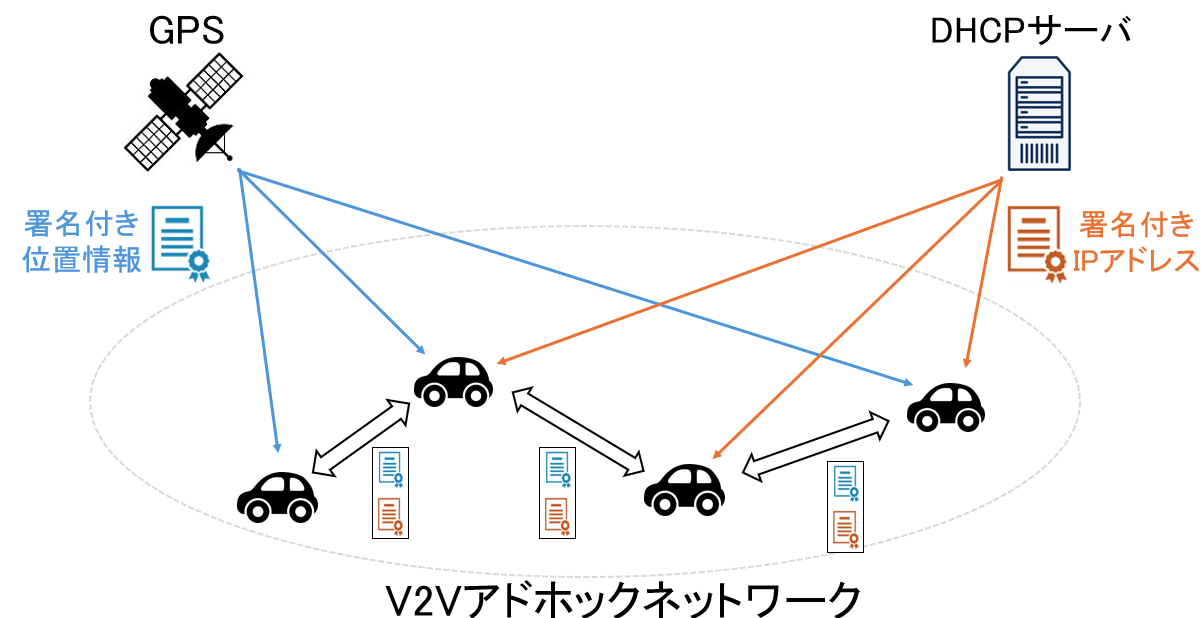
\includegraphics[scale=0.8]{figures/introduce.png}
  \caption{デジタル署名を用いた認証機構}
  \label{fig:introduce}
\end{figure}


